\documentclass[../thesis.tex]{subfiles}
% Separate preamble for this subfile. This preamble is loaded last, so one can override various functions before \begin{document}

% Better comment extension for Vscode colors these comments differently
% Normal comment color
% * Important information
% ! ALERT
% ? Question
% TODO stuff to do
% // This is strikethrough


\begin{document}

\begin{definition}[Lebesgue Space] % Heil REal analysis book page 269, citation?
    Let $E$ be a measurable subset of $\R^d$. Given $1 \leq p < \infty$ and a measurable function $f:E\rightarrow \C$, we say that $f$ is \emph{$p$-integrable} if the Lebesgue integral of $|f|^p$ is finite, that is
    \begin{equation*}
        \int_{E} |f(t)|^p dt < \infty,
    \end{equation*}
    where $dt= dt_1 \dots dt_d$. We define the \emph{Lebesgue space} $L^p(E)$ as the set of all $p$-integrable functions on $E$, and equip it with the norm
    \begin{equation*}
        \bral{f}_{L^p(E)} = \bracMed{\int_{E} |f(t)|^p dt}^{1/p}. \qedhere
    \end{equation*}
\end{definition}

%! \colorbox{BurntOrange}{Overgang} Synes det trengs overgang her. Of all the $L^p$ spaces, the case $p=2$ is special since $L^2(E)$ is the only space whose norm
The case where $p=2$ is special since $L^2(E)$ is the only $L^p$ space whose norm is induced from the inner product
\begin{equation*}
    \braaMed{f, g}_{L^2(E)} = \int_{E} f(t)\overline{g(t)} dt,
\end{equation*}
for two functions $f,g\in L^2(E)$. By the Riesz-Fischer theorem \cite[p.~279]{heilIntroductionRealAnalysis2019}, all $L^p$ spaces are complete with respect to the \LPnorm. Hence, $L^2(E)$ is a Hilbert space. 

%! \colorbox{BurntOrange}{Overgang} Synes det trengs overgang her
%* —————————————————————————————————————— C Cont. FUNCTIONS ——————————————————————————————————————
Let
\begin{equation*}
    C([a,b]) = \braq{f:[a,b] \rightarrow \mathbb{C}: f \text{ is continuous on } [a,b]}
\end{equation*}
denote the set of all continuous, scalar-valued functions whose domain is the closed and bounded interval $\bras{a,b}$. The following useful result with proof can be found in \cite[p.~326]{rudinPrinciplesMathematicalAnalysis20}. 
\begin{lemma}\label{lem:c_dense_L2}
    The set of all continuous functions $C([a,b])$ is dense in the space $L^2([a,b])$ with respect to the \Ltwonorm.
\end{lemma}

%* —————————————————————————————————————— C PERIODIC FUNCTIONS ——————————————————————————————————————
Similarly, let 
\begin{equation*}
    \Cper([a,b])= \braqMed{f \in C[a,b]: f(a)=f(b)}
\end{equation*}
denote the set of all continuous, real-valued functions on the interval $\bras{a,b}$ satisfying $f(a)=f(b)$. It is periodic in the sense that each element $f$ can be extended to the whole real line by setting 
\begin{equation*}
    f(t+Pn) = f(t), \quad t\in \bras{a,b},
\end{equation*}
for $n\in \Z$ and $P=b-a$. We say that the extended function $f$ is $P$\emph{-periodic} as it repeats after $P$ units, meaning
\begin{equation*}
    f(t+P) = f(t), \quad t\in \R.
\end{equation*}
The converse is also true, meaning we have a one-to-one correspondence between elements of $\Cper([a,b])$ and functions that are $P$-periodic on the real line. % if $f'$ is a $P$-periodic function on $\R$, then when $f'$ is restricted to the domain $\bras{a,b}$ it is also an element of $\Cper([a,b])$.
Equivalently to \cref{lem:c_dense_L2}, we have a similar \namecref{lem:c_per_dense_c_and_dense_L2} for $\Cper([a,b])$, and note that the proof closely follows the one by Heil in \cite[p.~228]{heilMetricsNormsInner2018}.  % although it is never explicitly stated.
\begin{lemma}\label{lem:c_per_dense_c_and_dense_L2}
    The set of all periodic functions $\Cper([a,b])$ is dense in the space $L^2([a,b])$ with respect to the \Ltwonorm.
\end{lemma}
%* The proof of \cref{lem:c_per_dense_c_and_dense_L2} closely follows the proof by Heil in \cite[p.~228]{heilMetricsNormsInner2018} although it is never explicitly stated. 
%Although not stated as explicitly as a result, the proof of \cref{lem:c_per_dense_c_and_dense_L2} can be found in \cite[p.~228]{heilMetricsNormsInner2018}.
\begin{proof}
    \begin{figure}
        \centering
        %\includegraphics[width=0.45\textwidth]{cper_dense_c.png}
        

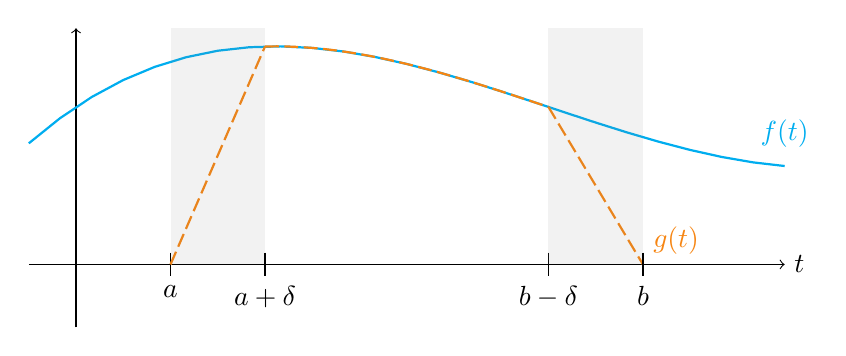
\begin{tikzpicture}[xscale=6,yscale=2]
    %* Draw axes
    \draw[->] (-0.1,0) -- (1.5,0) node[right] {$t$};  % går fra -0.3 til 1.5 på X aksen
    \draw[->] (0,-0.4) -- (0,1.5); %node[above] {$y$};  % går fra -0.4 til 1.5 på Y aksen
    
    %* Plot polynomial function
    \draw[cyan, thick, domain = -0.1:1.5] plot (\x, {(\x-1)^3 - (\x-1) + 1}) node[above, yshift=1mm] {$f(t)$};


    %* Draw labeled marks on the x-axis
    \foreach \x in { 0.2 }{
        \draw (\x,0.075) -- (\x,-0.075) node[below] {$a$}; % Lengden på linjen først
        %\draw[dashed] (\x,0) -- (\x,1.5);
        \draw[BurntOrange, dash pattern={on 5pt off 2pt}, thick] (\x,0) -- (0.4,{(0.4-1)^3 - (0.4-1) + 1});  % end value is the function value
    }

    %* Shade area between the points above and below
    \fill[gray, opacity=0.1] (0.2,0) -- (0.2,1.5) -- (0.4,1.5) -- (0.4,0) -- cycle;
    %\draw[pattern={north east lines},pattern color=gray] (0.2,0) rectangle +(0.2,1.5);

    %* Draw labeled marks on the x-axis
    \foreach \x in { 0.4 }{
        \draw (\x,0.075) -- (\x,-0.075) node[below] {$a+\delta$}; % Lengden på linjen først
        %\draw[dashed] (\x,0) -- (\x,1.5);
    }

    %* draw the middle parts of the approximating function g  —————— MIDDLE ——————
    %\draw[red, thick, dashed, domain=0.4:1] plot (\x, {(\x-1)^3 - (\x-1) + 1}) node[anchor=south east, yshift=2mm] {$g(t)$};
    %\draw[BurntOrange, thick, dashed, domain=0.4:1] plot (\x, {(\x-1)^3 - (\x-1) + 1});
    \draw[BurntOrange, thick, dash pattern={on 5pt off 2pt}, domain=0.4:1] plot (\x, {(\x-1)^3 - (\x-1) + 1});
    

    %* Draw labeled marks on the x-axis
    \foreach \x in { 1 }{
        \draw (\x,0.075) -- (\x,-0.075) node[below] {$b-\delta$}; % Lengden på linjen først
        %\draw[dashed] (\x,0) -- (\x,1.5);
        \draw[BurntOrange, dash pattern={on 5pt off 2pt}, thick] (\x,{(\x-1)^3 - (\x-1) + 1}) -- (1.2,0) node[anchor=south west, yshift=0mm] {$g(t)$};  % end value is the function value
    }

    %* Shade area between the points above and below
    \fill[gray, opacity=0.1] (1,0) -- (1,1.5) -- (1.2,1.5) -- (1.2,0) -- cycle;

    %* Draw labeled marks on the x-axis
    \foreach \x in { 1.2 }{
        \draw (\x,0.075) -- (\x,-0.075) node[below] {$b$};
        %\draw[dashed] (\x,0) -- (\x,1.5);
    }

    %\fill[gray, opacity=0.3] (0.2,0) -- (0.2,{(0.2-1)^3 - (0.2-1) + 1}) -- (0.4,{(0.4-1)^3 - (0.4-1) + 1}) -- (0.4,0) -- cycle;

\end{tikzpicture}


\mycomment{  %! Whole middle fill with dotted lines
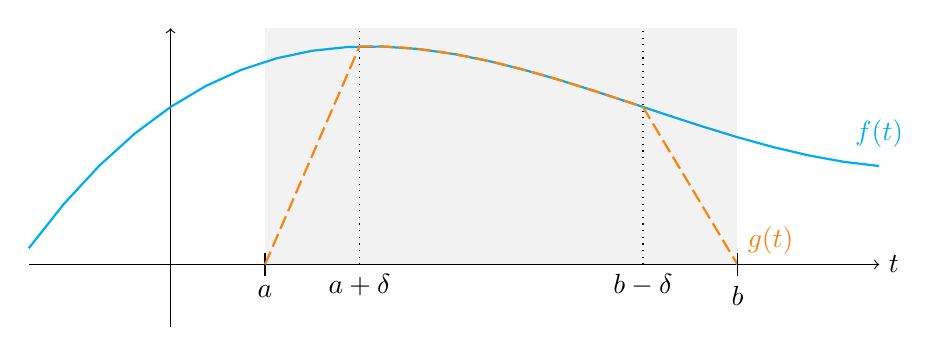
\begin{tikzpicture}[xscale=6,yscale=2]
    %* Draw axes
    \draw[->] (-0.3,0) -- (1.5,0) node[right] {$t$};  % går fra -0.3 til 1.5 på X aksen
    \draw[->] (0,-0.4) -- (0,1.5); %node[above] {$y$};  % går fra -0.4 til 1.5 på Y aksen
    
    %* Plot polynomial function
    \draw[cyan, thick, domain=-0.3:1.5] plot (\x, {(\x-1)^3 - (\x-1) + 1}) node[above, yshift=1mm] {$f(t)$};
    %* Shade area 
    \fill[gray, opacity=0.1] (0.2,0) -- (0.2,1.5) -- (1.2,1.5) -- (1.2,0) -- cycle;

    %* Draw labeled marks on the x-axis
    \foreach \x in { 0.2 }{
        \draw (\x,0.075) -- (\x,-0.075) node[below] {$a$}; % Lengden på linjen først
        %\draw[dashed] (\x,0) -- (\x,1.5);
        \draw[BurntOrange, dash pattern={on 5pt off 2pt}, thick] (\x,0) -- (0.4,{(0.4-1)^3 - (0.4-1) + 1});  % end value is the function value
    }

    %* Draw labeled marks on the x-axis
    \foreach \x in { 0.4 }{
        \draw (\x,0) -- (\x,-0.001) node[below] {$a+\delta$}; % Lengden på linjen først
        \draw[dotted] (\x,0) -- (\x,1.5);
    }

    %* draw the middle parts of the approximating function g  —————— MIDDLE ——————
    %\draw[red, thick, dashed, domain=0.4:1] plot (\x, {(\x-1)^3 - (\x-1) + 1}) node[anchor=south east, yshift=2mm] {$g(t)$};
    %\draw[BurntOrange, thick, dashed, domain=0.4:1] plot (\x, {(\x-1)^3 - (\x-1) + 1});
    \draw[BurntOrange, thick, dash pattern={on 5pt off 2pt}, domain=0.4:1] plot (\x, {(\x-1)^3 - (\x-1) + 1});
    

    %* Draw labeled marks on the x-axis
    \foreach \x in { 1 }{
        \draw (\x,0) -- (\x,-0.001) node[below] {$b-\delta$}; % Lengden på linjen først
        \draw[dotted] (\x,0) -- (\x,1.5);
        \draw[BurntOrange, dash pattern={on 5pt off 2pt}, thick] (\x,{(\x-1)^3 - (\x-1) + 1}) -- (1.2,0) node[anchor=south west, yshift=0mm] {$g(t)$};  % end value is the function value
    }


    %* Draw labeled marks on the x-axis
    \foreach \x in { 1.2 }{
        \draw (\x,0.075) -- (\x,-0.075) node[below] {$b$};
        %\draw[dashed] (\x,0) -- (\x,1.5);
    }

    %\fill[gray, opacity=0.3] (0.2,0) -- (0.2,{(0.2-1)^3 - (0.2-1) + 1}) -- (0.4,{(0.4-1)^3 - (0.4-1) + 1}) -- (0.4,0) -- cycle;

\end{tikzpicture}
}

\mycomment{  %! Whole middle fill with dashed lines
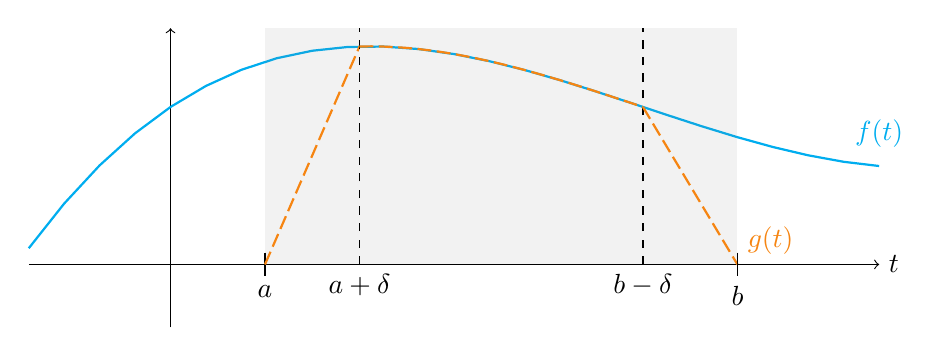
\begin{tikzpicture}[xscale=6,yscale=2]
    %* Draw axes
    \draw[->] (-0.3,0) -- (1.5,0) node[right] {$t$};  % går fra -0.3 til 1.5 på X aksen
    \draw[->] (0,-0.4) -- (0,1.5); %node[above] {$y$};  % går fra -0.4 til 1.5 på Y aksen
    
    %* Plot polynomial function
    \draw[cyan, thick, domain=-0.3:1.5] plot (\x, {(\x-1)^3 - (\x-1) + 1}) node[above, yshift=1mm] {$f(t)$};
    %* Shade area 
    \fill[gray, opacity=0.1] (0.2,0) -- (0.2,1.5) -- (1.2,1.5) -- (1.2,0) -- cycle;

    %* Draw labeled marks on the x-axis
    \foreach \x in { 0.2 }{
        \draw (\x,0.075) -- (\x,-0.075) node[below] {$a$}; % Lengden på linjen først
        %\draw[dashed] (\x,0) -- (\x,1.5);
        \draw[BurntOrange, dash pattern={on 5pt off 2pt}, thick] (\x,0) -- (0.4,{(0.4-1)^3 - (0.4-1) + 1});  % end value is the function value
    }

    %* Draw labeled marks on the x-axis
    \foreach \x in { 0.4 }{
        \draw (\x,0) -- (\x,-0.001) node[below] {$a+\delta$}; % Lengden på linjen først
        \draw[dashed] (\x,0) -- (\x,1.5);
    }

    %* draw the middle parts of the approximating function g  —————— MIDDLE ——————
    %\draw[red, thick, dashed, domain=0.4:1] plot (\x, {(\x-1)^3 - (\x-1) + 1}) node[anchor=south east, yshift=2mm] {$g(t)$};
    %\draw[BurntOrange, thick, dashed, domain=0.4:1] plot (\x, {(\x-1)^3 - (\x-1) + 1});
    \draw[BurntOrange, thick, dash pattern={on 5pt off 2pt}, domain=0.4:1] plot (\x, {(\x-1)^3 - (\x-1) + 1});
    

    %* Draw labeled marks on the x-axis
    \foreach \x in { 1 }{
        \draw (\x,0) -- (\x,-0.001) node[below] {$b-\delta$}; % Lengden på linjen først
        \draw[dashed] (\x,0) -- (\x,1.5);
        \draw[BurntOrange, dash pattern={on 5pt off 2pt}, thick] (\x,{(\x-1)^3 - (\x-1) + 1}) -- (1.2,0) node[anchor=south west, yshift=0mm] {$g(t)$};  % end value is the function value
    }


    %* Draw labeled marks on the x-axis
    \foreach \x in { 1.2 }{
        \draw (\x,0.075) -- (\x,-0.075) node[below] {$b$};
        %\draw[dashed] (\x,0) -- (\x,1.5);
    }

    %\fill[gray, opacity=0.3] (0.2,0) -- (0.2,{(0.2-1)^3 - (0.2-1) + 1}) -- (0.4,{(0.4-1)^3 - (0.4-1) + 1}) -- (0.4,0) -- cycle;

\end{tikzpicture}
}


\mycomment{  %! Whole middle fill with dashed lines and solid lines at the end
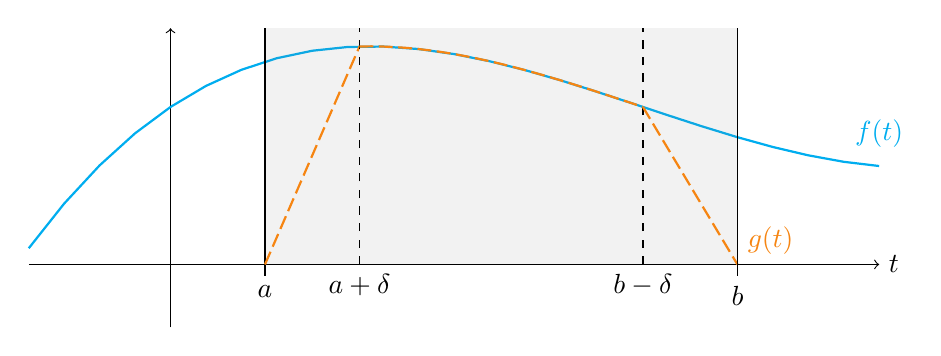
\begin{tikzpicture}[xscale=6,yscale=2]
    %* Draw axes
    \draw[->] (-0.3,0) -- (1.5,0) node[right] {$t$};  % går fra -0.3 til 1.5 på X aksen
    \draw[->] (0,-0.4) -- (0,1.5); %node[above] {$y$};  % går fra -0.4 til 1.5 på Y aksen
    
    %* Plot polynomial function
    \draw[cyan, thick, domain=-0.3:1.5] plot (\x, {(\x-1)^3 - (\x-1) + 1}) node[above, yshift=1mm] {$f(t)$};
    %* Shade area 
    \fill[gray, opacity=0.1] (0.2,0) -- (0.2,1.5) -- (1.2,1.5) -- (1.2,0) -- cycle;

    %* Draw labeled marks on the x-axis
    \foreach \x in { 0.2 }{
        \draw (\x,0.075) -- (\x,-0.075) node[below] {$a$}; % Lengden på linjen først
        \draw(\x,0) -- (\x,1.5);
        \draw[BurntOrange, dash pattern={on 5pt off 2pt}, thick] (\x,0) -- (0.4,{(0.4-1)^3 - (0.4-1) + 1});  % end value is the function value
    }

    %* Draw labeled marks on the x-axis
    \foreach \x in { 0.4 }{
        \draw (\x,0) -- (\x,-0.001) node[below] {$a+\delta$}; % Lengden på linjen først
        \draw [dashed] (\x,0) -- (\x,1.5);
    }

    %* draw the middle parts of the approximating function g  —————— MIDDLE ——————
    %\draw[red, thick, dashed, domain=0.4:1] plot (\x, {(\x-1)^3 - (\x-1) + 1}) node[anchor=south east, yshift=2mm] {$g(t)$};
    %\draw[BurntOrange, thick, dashed, domain=0.4:1] plot (\x, {(\x-1)^3 - (\x-1) + 1});
    \draw[BurntOrange, thick, dash pattern={on 5pt off 2pt}, domain=0.4:1] plot (\x, {(\x-1)^3 - (\x-1) + 1});
    

    %* Draw labeled marks on the x-axis
    \foreach \x in { 1 }{
        \draw (\x,0) -- (\x,-0.001) node[below] {$b-\delta$}; % Lengden på linjen først
        \draw [dashed] (\x,0) -- (\x,1.5);
        \draw[BurntOrange, dash pattern={on 5pt off 2pt}, thick] (\x,{(\x-1)^3 - (\x-1) + 1}) -- (1.2,0) node[anchor=south west, yshift=0mm] {$g(t)$};  % end value is the function value
    }


    %* Draw labeled marks on the x-axis
    \foreach \x in { 1.2 }{
        \draw (\x,0.075) -- (\x,-0.075) node[below] {$b$};
        \draw (\x,0) -- (\x,1.5);
    }

    %\fill[gray, opacity=0.3] (0.2,0) -- (0.2,{(0.2-1)^3 - (0.2-1) + 1}) -- (0.4,{(0.4-1)^3 - (0.4-1) + 1}) -- (0.4,0) -- cycle;

\end{tikzpicture}
}
        \caption{The approximation of the continuous function $f(t)$ in a solid blue by a periodic function $g(t)$ in dashed orange.}
        \label{fig:g_periodic_close_to_f}
    \end{figure}
    %Since $C([a,b])$ is dense in $L^2([a,b])$ from \cref{lem:c_dense_L2}, it will then follow that $\Cper([a,b])$ is dense in $L^2([a,b])$ if we can show that $\Cper([a,b])$ is dense in $C([a,b])$.
    %If we can show that $\Cper([a,b])$ is dense in $C([a,b])$, it will follow that $\Cper([a,b])$ is dense in $L^2([a,b])$, since we know from \cref{lem:c_dense_L2} that $C([a,b])$ is dense in $L^2([a,b])$. 
    If we can show that $\Cper([a,b])$ is dense in $C([a,b])$, it will follow from \cref{lem:c_dense_L2} that $\Cper([a,b])$ is dense in $L^2([a,b])$, since $C([a,b])$ is dense in $L^2([a,b])$. Let $f \in C([a,b])$, $\varepsilon>0$ and $\delta = \varepsilon^2/(8\|f\|_\infty)$. We aim to construct a piecewise continuous function $g$ which is identical to $f$ on the interval $[a+\delta,b-\delta ]$ and which attains the value $g = 0$ at the endpoints, making $g\in \Cper([a,b])$. We will see that this will change the \Ltwonorm \space by a negligible amount. In other words, this allows us to approximate any continuous function as closely as we want by a modified (periodic) version of the original function. We construct $g$ in the following way  %. We will see that this will change the \Ltwonorm \space by a negligible amount and only at the expense of two intervals of length $\delta$
    \begin{equation*} % kan lage formel for g på ax+b formel: dvs $dy/dx \cdot x + b$ ELLER  $ -g(b-\delta) / \delta \cdot x + g(b-\delta)/ \delta $ <- dette er høyre side.
        g(t) = 
        \begin{cases} a, &  t=a,\\  
            \text{linear}, &  0<t<a+\delta,\\ 
            f(t), & a+\delta \leq t \leq b-\delta,\\ 
            \text{linear}, &  b-\delta <t<b,\\ 
            a, &  t=b,
        \end{cases}
    \end{equation*} 
    as illustrated in \cref{fig:g_periodic_close_to_f}. Observe that for all $t$ on the interval $[a+\delta, b-\delta]$ we have $|f(t)-g(t)|= 0$, and for all other values of $t$ we know that
    \begin{equation*}
        |g(t)| \leq \|g\|_{\infty} = \sup_{t\in[a,b]} |g(t)| = \sup_{t\in[a+\delta, b-\delta]} |g(t)| = \sup_{t\in[a+\delta, b-\delta]} |f(t)| \leq \sup_{t\in[a, b]} |f(t)| =\| f\|_{\infty}
    \end{equation*}
    with equality in the third step using the fact that $g$ is linear and goes towards zero as it approaches $0$ or $b$, and therefore attains its greatest value on the interval $[a+\delta,b-\delta]$ where it is equal to $f$. Using this, as well as the triangle inequality, we have that
    \begin{equation*}
        \left|f(t)-g(t) \right| \leq |f(t)| + |-g(t)| \leq \|f \|_{\infty} + \|f \|_{\infty} = 2 \|f \|_{\infty}
    \end{equation*}
    for all $t$ on the intervals $[a, a+\delta]$ and $[b-\delta,b]$. Now,
    \begin{align*}
        \| f-g \|_{L^2}^2 &=  \int_0^{a+\delta} \left|f(t)-g(t) \right|^2dt + \int_{a+\delta}^{b-\delta} \left|f(t)-g(t) \right|^2dt +\int_{b-\delta}^{b} \left|f(t)-g(t) \right|^2dt\\ 
        &\leq \int_0^{a+\delta} (2 \| f\|_\infty)^2dt + 0 +\int_{b-\delta}^{b} (2 \| f\|_\infty)^2dt\\
        &=  4 \delta \| f\|_\infty^2 + 4 \delta \| f\|_\infty^2\\ 
        &= \varepsilon^2
    \end{align*}
    This shows that $\Cper([a,b])$ is dense in $C([a,b])$, which finalizes our proof.
\end{proof}

%* —————————————————————————————————————— Indicator function  ——————————————————————————————————————
\begin{definition}(Indicator function)\label{def:indicator}
    Let $E$ be a subset of a set $X$. The \emph{indicator function}, also known as the \emph{characteristic function} of $E$, is a function $\indicator{E}{t}: X \rightarrow \braq{0,1}$ where
    \begin{equation*}
        \indicator{E}{t}  = 
        \begin{cases} 
            1, &  t\in E,\\
            0, &  t \notin E.
        \end{cases}
        \qedhere
    \end{equation*}
\end{definition}


\begin{definition}\label{def:dot_prod}
    Let $t=(t_1,\dots t_d)$ and $\lambda=(\lambda_1, \dots, \lambda_d)$ be two vectors in $\R^d$. The inner product, denoted $\langle \cdot, \cdot \rangle$, between $t$ and $\lambda$ is
    \begin{equation*}
        \langle t, \lambda \rangle = \sum_{n=1}^d t_n \lambda_n = t_1\lambda_1 + \dots + t_d\lambda_d,
    \end{equation*}
    also known as the dot product. 
\end{definition}


\end{document}